
\documentclass[codesnippet,nojss]{jss}\usepackage[]{graphicx}\usepackage[]{color}
% maxwidth is the original width if it is less than linewidth
% otherwise use linewidth (to make sure the graphics do not exceed the margin)
\makeatletter
\def\maxwidth{ %
  \ifdim\Gin@nat@width>\linewidth
    \linewidth
  \else
    \Gin@nat@width
  \fi
}
\makeatother

\usepackage{Sweave}



%\VignetteEngine{knitr::knitr}
% \VignetteIndexEntry{Using sparseMVN}
%\VignetteKeyword{sparseMVN}

\usepackage[utf8]{inputenc}
\usepackage{amsmath}
\usepackage{amsfonts}
\usepackage{subcaption}
\usepackage{booktabs}
\usepackage{etoolbox}
\usepackage{placeins}
\usepackage{array}
\usepackage{tabularx}
\usepackage{multirow}

\newcommand{\func}[1]{\code{#1}}
\newcommand{\class}[1]{\textsl{#1}}
\newcommand{\funcarg}[1]{\code{#1}}
\newcommand{\variable}[1]{\code{#1}}
\newcommand{\Cond}[2]{\left.#1\,\middle|\,#2\right.}
\newcommand{\EV}[1]{\mathbf{E}\!\left(#1\right)}
\newcommand{\Var}[1]{\mathbf{var}\!\left(#1\right)}
\newcommand{\dist}[2]{#1\!\left(#2\right)}
\newcommand{\Logit}[1]{\logit\!\left(#1\right)}
\newcommand{\Cov}[1]{\mathbf{cov}\!\left(#1\right)}
\newcommand{\Norm}[1]{\mathbf{N}\!\left(#1\right)}
\newcommand{\MVN}[1]{\mathbf{MVN}\!\left(#1\right)}
\newcommand{\Real}[1]{\mathbb{R}^{#1}}
\newcommand{\bigO}[1]{\mathcal{O}\!\left(#1\right)}
\newcommand{\Mat}[1]{\mathbf{#1}}

\hyphenation{dCHMsimple}


 \author{Michael Braun\\Edwin L. Cox School of Business\\Southern Methodist University}
\Plainauthor{Michael Braun}
\title{\pkg{sparseMVN}: An R Package for Multivariate Normal Functions
  with Sparse Covariance and Precision Matrices}
\Plaintitle{sparseMVN: An R Package for Sparse MVN Functions}
\Shorttitle{sparseMVN}
\Keywords{multivariate normal, sparse matrices, covariance, simulation}
\Address{
  Michael Braun\\
  Edwin L. Cox School of Business\\
  Southern Methodist University\\
  6212 Bishop Blvd.\\
  Dallas, TX 75275\\
  E-mail:  \email{braunm@smu.edu}\\
  URL:  \url{http://www.smu.edu/Cox/Departments/FacultyDirectory/BraunMichael}
}


\Abstract{
The number of elements in a multivariate normal (MVN) covariance or
precision matrix grows quadratically in the number of variables.
Thus, sampling from, and computing densities of, an MVN random variable
is not scalable when all matrix elements are stored as a dense R matrix, but
may be when the matrix is sparse, and stored in a suitable compressed
format.  This package provides standard MVN sampling and density
algorithms that are optimized for sparse covariance and precision matrices.
}

\date{April 7, 2017}

%% need no \usepackage{Sweave.sty}
\IfFileExists{upquote.sty}{\usepackage{upquote}}{}
\begin{document}



The \pkg{mvtnorm} package \citep{R_mvtnorm} provides the
\func{dmvnorm} function to compute the density of a multivariate
normal (MVN) distributon, and
the \func{rmvnorm} function to simulate
MVN random variables.  These functions require the user to supply a
full, ``dense''
covariance matrix; if starting with a precision matrix, the user must first invert it explicitly.
This covariance matrix is
dense in the sense that, for an $M$-dimensional MVN random
variable, all $M^2$ elements are stored, so memory
requirements grow quadratically with the size of the problem.
Internally, both functions factor the covariance matrix using a
Cholesky decomposition, whose complexity is
$\bigO{M^3}$\citep{GolubVanLoan1996}.\footnote{\func{dmvnorm} has options for eigen and
  singular value decompositions. These are both $\bigO{M^3}$ as well.}  This
factorization is performed every time the function is called, even if
the covariance matrix does not
change from call to call.  Also, \func{rmvnorm} involves
multiplication of a triangular matrix, and \func{dmvnorm} involves
solving a triangular linear system.  Both of these operations are
$\bigO{M^2}$ \citep{GolubVanLoan1996} on dense matrices.  MVN
functions in other packages, such as \pkg{MASS} \citep{R_MASS} and \pkg{LaplacesDemon}
\citep{R_LaplacesDemon}, face similar
limitations.\footnote{\pkg{LaplacesDemon} does offer options for the user to supply pre-factored
covariance and precision matrices.  This avoids repeated calls to the $\bigO{M^3}$
factorization step, but not the $\bigO{M^2}$ matrix multiplication and
linear system solution steps.}  Thus, existing tools for working with
the MVN distribution in \proglang{R} are not practical for
high-dimensional MVN random variables.

However, for many applications the
covariance or precision matrix is sparse, meaning that the proportion
of nonzero elements is small, relative to the total size of the
matrix. The functions in the \pkg{sparseMVN} package exploit that
sparsity to reduce memory requirements, and to gain computational
efficiencies.  The \func{dmvn.sparse} function computes the MVN
density, and the \func{rmvn.sparse} function samples from an MVN
random variable.  Instead of requiring the
user to supply a dense covariance matrix, \func{dmvn.sparse} and
\func{rmvn.sparse} accept a pre-computed Cholesky decomposition of either the
covariance or precision matrix in a compressed sparse format. This
approach has several advantages:

\begin{enumerate}
\item Memory requirements are smaller because only the nonzero
  elements of the matrix are stored in a compressed sparse format.
\item Linear algebra algorithms that are optimzed for sparse matrices
  are more efficient because they avoid operations on matrix elements that are known to be zero.
\item When the precision matrix is initially available,
  there is no need to invert it into a covariance matrix explicitly.
  This feature of \pkg{sparseMVN} preserves sparsity, because the inverse of a sparse matrix is
  not necessarily sparse.
\item The Cholesky factor of the matrix is computed once, before the
  first \pkg{sparseMVN} function call, and is not repeated with subsequent calls
  (as long as the matrix does not change).
\end{enumerate}


The functions in \pkg{sparseMVN} rely on sparse matrix classes and
functions defined in the \pkg{Matrix} package
\citep{R_Matrix}.  The user creates the covariance or precision matrix
as a sparse, symmetric \class{dsCMatrix} matrix, and computes the
sparse Cholesky factor using the \func{Cholesky} function. Other than ensuring that
the factor for the covariance or precision matrix is in the correct
format, the \pkg{sparseMVN} functions behave
in much the same way as the corresponding \pkg{mvtnorm} functions.
Internally, \pkg{sparseMVN} uses
standard methods of computing the MVN density and simulating MVN
random variables (see Section \ref{sec:algorithms}).  Since a large
proportion of elements in the matrix are zero, we need
to store only the row and column indices, and the values, of the
unique nonzero elements.  The efficiency gains in \pkg{sparseMVN} come from
storing the covariance or precision matrix in a compressed format without
explicit zeros, and applying linear algebra routines that are
optimized for those sparse matrix structures.  The \pkg{Matrix}
package calls sparse linear algebra routines that are implemented in
the \pkg{CHOLMOD} library
\citep{ChenDavis2008,DavisHager1999,DavisHager2009}.



\section{Background}
Let $x\in\Real{M}$ be a realization of random variable
$X\sim\MVN{\mu,\Sigma}$, where $\mu\in\Real{M}$ is a vector,
$\Sigma\in\Real{M\times M}$ is a positive-definite covariance matrix,
and $\Sigma^{-1}\in\Real{M\times M}$ is a positive-definite precision matrix.

The log probability density of $x$ is

\begin{align}
\log f(x)&=-\frac{1}{2}\left(M \log (2\pi) + \log|\Sigma|
  +z^\top z\right),\quad\text{where}~z^\top z=\left(x-\mu\right)^\top\Sigma^{-1}\left(x-\mu\right)
 \end{align}

\subsection{MVN density computation and random number generation}\label{sec:algorithms}

The two computationally intensive steps in evaluating $\log f(x)$ are
computing $\log|\Sigma|$, and $z^\top z$, \emph{without} explicitly
inverting $\Sigma$ or repeating mathematical operations.  How one
performs these steps \emph{efficiently} in practice depends on whether the
covariance matrix $\Sigma$, or the precision matrix $\Sigma^{-1}$ is
available. For both cases, we start by finding a lower triangular matrix root:
$\Sigma=LL^\top$ or $\Sigma^{-1}=\Lambda\Lambda^\top$.  Since $\Sigma$
and $\Sigma^{-1}$ are positive definite, we will use the Cholesky
decomposition, which is the unique matrix root with all positive
elements on the diagonal.

With the Cholesky decomposition in hand, we compute the log
determinant of $\Sigma$ by adding the logs of the diagonal elements of
the factors.
\begin{align}
  \label{eq:logDet}
  \log|\Sigma|= \begin{cases}
    \phantom{-}2\sum_{m=1}^M\log L_{mm}&\text{ when $\Sigma$ is given}\\
    -2\sum_{m=1}^M\log \Lambda_{mm}&\text{ when $\Sigma^{-1}$ is given}
    \end{cases}
\end{align}

Having already computed the triangular matrix roots also speeds up the computation of
$z^\top z$.  If $\Sigma^{-1}$ is given, $z=\Lambda^\top(x-\mu)$ can be computed
efficiently as the product of an upper triangular matrix and a
vector. When $\Sigma$ is given, we find $z$ by solving the lower
triangular system $Lz=x-\mu$.  The subsequent $z^\top z$
computation is trivially fast.

The algorithm for simulating  $X\sim\MVN{\mu,\Sigma}$ also
depends on whether
$\Sigma$ or $\Sigma^{-1}$ is given.  As above, we start by computing
the Cholesky decomposition of the given covariance or precision
matrix. Define a random variable $Z\sim\MVN{0,I_M}$, and generate a realization
$z$ as a vector of $M$ samples from a standard normal distribution.  If $\Sigma$ is given,
then evaluate $x=Lz+\mu$.  If $\Sigma^{-1}$ is given, then solve for $x$ in the
triangular linear system $\Lambda^\top\left(x-\mu\right)=z$. The
resulting $x$ is a sample from $\MVN{\mu,\Sigma}$.  We confirm the
mean and covariance of $X$ as follows:
 \begin{align}
 \EV{X}&=\EV{LZ+\mu}=\EV{\Lambda^\top Z+\mu}=\mu\\
   \Cov{X}&= \Cov{LZ+\mu}=\EV{LZZ^\top L^\top}=LL^\top=\Sigma\\
     \Cov{X}&=\Cov{\Lambda^{\top^{-1}}Z+\mu}=\EV{\Lambda^{\top^{-1}}ZZ^\top\Lambda^{-1}}
     =\Lambda^{\top^{-1}}\Lambda^{-1}=(\Lambda\Lambda^\top)^{-1}=\Sigma
 \end{align}

These algorithms apply when the covariance/precision matrix is either
sparse or dense.  When the matrix is dense, the computational
complexity is $\bigO{M^3}$  for a Cholesky decomposition, and
$\bigO{M^2}$ for either solving the triangular linear
system or multiplying a triangular matrix by another matrix
\citep{GolubVanLoan1996}.  Thus, the computational cost grows
cubically with $M$ before the decomposition step, and quadratically if
the decomposition has already been completed.  Additionally, the storage
requirement for $\Sigma$ (or $\Sigma^{-1}$) grows quadratically with $M$.



\subsection{Sparse matrices in R}\label{sec:sparse}

The \pkg{Matrix} package \citep{R_Matrix} defines
various classes for storing sparse matrices in compressed formats. The
most important class for our purposes is
\class{dsCMatrix}, which defines a symmetric matrix, with numeric
(double precision) elements, in a column-compressed format.  Three
vectors define the underlying matrix:
the unique nonzero values (just one triangle is needed), the indices
in the value vector for the first value in each column, and the indices of the rows in
which each value is located. The storage requirements
for a sparse $M\times M$ symmetric matrix with $V$ unique nonzero
elements in one triangle are for $V$ double precision numbers, $V+M+1$ integers, and
some metadata.  In contrast, a dense representation of the same matrix
stores $M^2$ double precision values, regardless of symmetry and the number of
zeros. If $V$ grows more slowly than $M^2$, the matrix becomes
increasingly sparse (a smaller percentage of elements are nonzero),
with greater efficiency gains from storing the matrix in a
compressed sparse format.

\subsubsection{An example}

To illustrate how sparse matrices require less memory resources when
compressed than when stored densely, consider the following example,
which borrows heavily from the vignette of the
\pkg{sparseHessianFD} package \citep{R_sparseHessianFD}.

Suppose we have a dataset of $N$ households, each with $T$
 opportunities to purchase a particular product.  Let $y_i$ be the
 number of times household $i$ purchases the product, out of the $T$
 purchase opportunities, and let $p_i$ be the probability of
 purchase.  The heterogeneous parameter $p_i$ is the same for all $T$
 opportunities, so $y_i$ is a binomial random variable.

 Let $\beta_i\in\Real{k}$ be a heterogeneous coefficient vector that
 is specific to household $i$, such that
 $\beta_i=(\beta_{i1},\dotsc,\beta_{ik})$. Similarly,
 $w_i\in\Real{k}$ is a vector of household-specific covariates. Define each
 $p_i$ such that the log odds of $p_i$ is a linear function of
 $\beta_i$ and $w_i$, but does not depend directly on $\beta_j$ and $w_j$ for
 another household $j\neq i$.
\begin{align}
  p_i=\frac{\exp(w_i'\beta_i)}{1+\exp(w_i'\beta_i)},~i=1 ... N
\end{align}

The coefficient vectors $\beta_i$ are distributed across the population of households
following a MVN distribution with mean $\mu\in\Real{k}$ and
covariance $\Mat{A}\in\Real{k\times k}$.   Assume that we know
$\Mat{A}$, but not $\mu$, so we place a multivariate normal prior
on $\mu$, with mean $0$ and
covariance $\Mat{\Omega}\in\Real{k\times k}$.  Thus, the parameter
vector $x\in\Real{(N+1)k}$ consists of the $Nk$ elements in the $N$ $\beta_i$ vectors,
and the $k$ elements in $\mu$.

The log posterior density, ignoring any normalization constants, is
\begin{align}
  \label{eq:LPD}
  \log \pi(\beta_{1:N},\mu|\Mat{Y}, \Mat{W}, \Mat{A},\Mat{\Omega})=\sum_{i=1}^N\left(p_i^{y_i}(1-p_i)^{T-y_i}
  -\frac{1}{2}\left(\beta_i-\mu\right)^\top\Mat{A}^{-1}\left(\beta_i-\mu\right)\right)
-\frac{1}{2}\mu^\top\Mat{\Omega}^{-1}\mu
\end{align}

Because one element of $\beta_i$ can be correlated with another
element of $\beta_i$ (for the same unit), we allow for the
cross-partials between elements of $\beta_i$ for any $i$ to be
nonzero.  Also, because the mean of each $\beta_i$ depends on $\mu$,
the cross-partials between $\mu$ and any $\beta_i$ can be nonzero.
However, since the $\beta_i$ and $\beta_j$ are independent samples,
and the $y_i$ are
conditionally independent, the cross-partial derivatives between an
element of $\beta_i$ and any element of any $\beta_j$ for $j\neq i$,
must be zero.  When $N$ is much greater than $k$, there will be many
more zero cross-partial derivatives than nonzero, and the Hessian of
the log posterior density will be sparse.



The sparsity pattern depends on how the variables are
ordered. One such ordering is to group all of the
coefficients in the $\beta_i$ for each unit together, and place $\mu$
at the end.
\begin{align}
\beta_{11},\dotsc,\beta_{1k},\beta_{21},\dotsc,\beta_{2k},~\dotsc~,\beta_{N1},\dotsc,\beta_{Nk},\mu_1,\dotsc,\mu_k
\end{align}
In this case, the Hessian has a ``block-arrow'' pattern.  Figure
\ref{fig:blockarrow} illustrates this pattern for $N=5$
and $k=2$ (12 total
variables).

Another possibility is to group coefficients for each covariate
together.
\begin{align}
\beta_{11},\dotsc,\beta_{N1},\beta_{12},\dotsc,\beta_{N2},~\dotsc~,\beta_{1k},\dotsc,\beta_{Nk},\mu_1,\dotsc,\mu_k
\end{align}
Now the Hessian has an "banded" sparsity pattern, as in Figure~\ref{fig:banded}.

\begin{figure}[tbp]\centering
   \begin{subfigure}[b]{.5\textwidth}
\begin{Schunk}
\begin{Soutput}

 [1,] | | . . . . . . . . | |
 [2,] | | . . . . . . . . | |
 [3,] . . | | . . . . . . | |
 [4,] . . | | . . . . . . | |
 [5,] . . . . | | . . . . | |
 [6,] . . . . | | . . . . | |
 [7,] . . . . . . | | . . | |
 [8,] . . . . . . | | . . | |
 [9,] . . . . . . . . | | | |
[10,] . . . . . . . . | | | |
[11,] | | | | | | | | | | | |
[12,] | | | | | | | | | | | |
\end{Soutput}
\end{Schunk}
\caption{A ``block-arrow'' sparsity pattern.}\label{fig:blockarrow}
\end{subfigure}%
\begin{subfigure}[b]{.5\textwidth}
\begin{Schunk}
\begin{Soutput}

 [1,] | . . . . | . . . . | |
 [2,] . | . . . . | . . . | |
 [3,] . . | . . . . | . . | |
 [4,] . . . | . . . . | . | |
 [5,] . . . . | . . . . | | |
 [6,] | . . . . | . . . . | |
 [7,] . | . . . . | . . . | |
 [8,] . . | . . . . | . . | |
 [9,] . . . | . . . . | . | |
[10,] . . . . | . . . . | | |
[11,] | | | | | | | | | | | |
[12,] | | | | | | | | | | | |
\end{Soutput}
\end{Schunk}
 \caption{A ``banded'' sparsity pattern.}\label{fig:banded}
\end{subfigure}
\caption{Two examples of sparsity patterns for a hierarchical model.}\label{fig:patterns}
\end{figure}




In both cases, the number of nonzeros is the same.  There are 144 elements in this symmetric matrix.  If the
matrix is stored in the standard \pkg{base} \proglang{R} dense
format, memory is reserved for all 144 values, even though only 64 values are
nonzero, and only 38 values are unique. For larger
matrices, the reduction in memory requirements by storing the matrix
in a sparse format can be substantial.\footnote{Because sparse matrix
  structures store row and column indices of the nonzero values, they
  may use more memory than dense storage if the total number of
  elements is small}. If $N=$1,000, then
$M=$2,002, with more than $4$ million
elements in the Hessian.  However, only 12,004 of those elements are
nonzero, with 7,003 unique values in the lower
triangle.  The dense
matrix requires 30.6 Mb of RAM,
while a sparse symmetric matrix of the \class{dsCMatrix} class requires only 91.6 Kb.

This example is relevant because, when evaluated at the posterior
mode, the Hessian matrix of the log posterior is the MVN precision
matrix $\Sigma^{-1}$ of a MVN approximatation to
the posterior distribution of $\left(\beta_{1:N},\mu\right)$. If we
were to simulate from this MVN using
\func{rmvnorm}, or evaluate MVN densities using \func{dmvnorm}, we
would need to invert $\Sigma^{-1}$ to $\Sigma$ first, and store it as
a dense matrix. Internally, \func{rmvnorm} and \func{dmvnorm} invoke
dense linear algebra routines, including matrix factorization.


\section{Using the sparseMVN package}

The signatures of the \pkg{sparseMVN} key sparse matrix functions are

\begin{Schunk}
\begin{Sinput}
rmvn.sparse(n, mu, CH, prec=TRUE)
dmvn.sparse(x, mu, CH, prec=TRUE, log=TRUE)
\end{Sinput}
\end{Schunk}

The \func{rmvn.sparse} function returns a matrix $x$ with \funcarg{n}
rows and \func{length(mu)} columns.  \func{dmvn.sparse} returns a
vector of length \funcarg{n}: densities if \funcarg{log=FALSE},
and log densities if \funcarg{log=TRUE}.



{\setlength{\extrarowheight}{.25em}
\begin{table}[ptb]
\begin{tabularx}{\linewidth}{>{\bfseries}r X}
  \toprule
  x& A numeric matrix.  Each row is an MVN sample.\\
  mu&A numeric vector.  The mean of the MVN random variable.\\
  CH&Either a \class{dCHMsimpl} or
      \class{dCHMsuper} object representing the Cholesky decomposition of
      the covariance/precision matrix.\\
  prec&Logical value that identifies CH as the Cholesky decomposition of
        either a covariance ($\Sigma$, \funcarg{prec=TRUE}) or
        precision($\Sigma^{-1}$, \funcarg{prec=FALSE}) matrix.\\
  n&Number of random samples to be generated.\\
  log&If \funcarg{log=TRUE}, the log density is returned.\\
 \bottomrule
\end{tabularx}
\caption{Arguments to the \func{rmvn.sparse} and \func{dmvn.sparse} functions.}\label{tab:args}
\end{table}
}

Table~\ref{tab:args} describes the function arguments. These functions do
require the user to compute the Cholesky decomposition \funcarg{CH} beforehand, but
this needs to be done only once (as long as $\Sigma$ or $\Sigma^{-1}$
does not change). \funcarg{CH}
should be computed using the \func{Cholesky} function from the
\pkg{Matrix} package. More details about the \func{Cholesky} function
are available in the \pkg{Matrix}
documentation, but it is a simple function to use.  The first
argument is a sparse symmetric matrix stored as a \class{dsCMatrix} object.
As far as we know, there is no
particular need to deviate from the defaults of the remaining
arguments.  If \func{Cholesky} uses a fill-reducing permutation to compute
\funcarg{CH}, the \pkg{sparseMVN} functions will handle that directly, with no
additional user intervention required.  The \func{chol} function in
\pkg{base} \proglang{R} should not be used.

\subsection{An example}\label{sec:example}

Suppose we want to generate samples from an MVN approximation to
the posterior distribution of our example model from Section \ref{sec:sparse}.  \pkg{sparseMVN} includes
functions to simulate data for the example (\func{binary.sim}), and to
compute the log
posterior density (\func{binary.f}), gradient (\func{binary.grad}),
and Hessian (\func{binary.hess}).  The \func{trust.optim}
function in the \pkg{trustOptim} package \citep{R_trustOptim} is a
nonlinear optimizer that estimates the curvature of the objective
function using a sparse Hessian.

\begin{Schunk}
\begin{Sinput}
R> D <- sparseMVN::binary.sim(N=50, k=2, T=50)
R> priors <- list(inv.A=diag(2), inv.Omega=diag(2))
R> start <- rep(c(-1,1),51)
R> opt <- trustOptim::trust.optim(start,
+                                fn=sparseMVN::binary.f,
+                                gr=sparseMVN::binary.grad,
+                                hs=sparseMVN::binary.hess,
+                                data=D, priors=priors,
+                                method="Sparse",
+                                control=list(function.scale.factor=-1))
\end{Sinput}
\end{Schunk}

The call to \func{trust.optim} returns the posterior mode, and the
Hessian evaluated at the mode. These results serve as the mean and the negative precision
of the MVN approximation to the posterior distribution of the model.

\begin{Schunk}
\begin{Sinput}
R> R <- 100
R> pm <- opt[["solution"]]
R> H <- -opt[["hessian"]]
R> CH <- Cholesky(H)
\end{Sinput}
\end{Schunk}

We can then sample from the posterior using an MVN approximation, and compute the MVN log density for each sample.

\begin{Schunk}
\begin{Sinput}
R> samples <- rmvn.sparse(R, pm, CH, prec=TRUE)
R> logf <- dmvn.sparse(samples, pm, CH, prec=TRUE)
\end{Sinput}
\end{Schunk}

The ability to accept a precision matrix, rather than having to invert
it to a covariance matrix, is a valuable feature of \pkg{sparseMVN}.
This is because the inverse of a sparse matrix is not necessarily
sparse. In the following chunk, we invert the Hessian, and drop zero
values to maintain any remaining sparseness. Note that there are
10,404 total elements in the Hessian.

\begin{Schunk}
\begin{Sinput}
R> Matrix::nnzero(H)
\end{Sinput}
\begin{Soutput}
# [1] 402
\end{Soutput}
\begin{Sinput}
R> Hinv <- drop0(solve(H))
R> Matrix::nnzero(Hinv)
\end{Sinput}
\begin{Soutput}
# [1] 10404
\end{Soutput}
\end{Schunk}

Nevertheless, we should check that the log densities from
\func{dmvn.sparse} correspond to those that we would get from \func{dmvnorm}.

\begin{Schunk}
\begin{Sinput}
R> logf_dense <- dmvnorm(samples, pm, as.matrix(Hinv), log=TRUE)
R> all.equal(logf, logf_dense)
\end{Sinput}
\begin{Soutput}
# [1] TRUE
\end{Soutput}
\end{Schunk}



\begin{Schunk}
\begin{Soutput}
# `summarise()` has grouped output by 'N', 'k', 'stat', 'pattern'. You can override using the `.groups` argument.
# `summarise()` has grouped output by 'N', 'k', 'stat', 'pattern'. You can override using the `.groups` argument.
\end{Soutput}
\end{Schunk}

\section{Timing}

In this section we show the efficiency gains from \pkg{sparseMVN} by comparing the run times between \func{rmvn.sparse} and
\func{rmvnorm}, and between \func{dmvn.sparse} and
\func{dmvnorm}.  In these tests, we construct covariance/precision
matrices with the same structure as the Hessian of the log posterior
density of the example model in Section \ref{sec:example}.  Parameters are
ordered such that the matrix has a block-arrow pattern, as in
Figure~\ref{fig:blockarrow}.  The size and sparsity of the test matrices
vary through manipulation of the number of blocks ($N$), the size of
each block ($k$), and the number of rows/columns in the margin (also $k$).  Each test matrix has
$(N+1)k$ rows and columns.  Table~\ref{tab:cases} summarizes the case
conditions.

\begin{table}\centering
  \begin{tabular}{rrrrrrr}
    \toprule
    &&&&\multicolumn{3}{c}{nonzeros}\\
    \cmidrule(lr){5-7}
    &$N$&variables&elements&full&lower tri&sparsity\\
    \midrule
% latex table generated in R 4.1.0 by xtable 1.8-4 package
% Fri Sep 24 11:19:18 2021
 \multirow{8}{*}{k=2} & 10 & 22 & 484 & 124 & 73 & 0.256 \\
   & 20 & 42 & 1,764 & 244 & 143 & 0.138 \\
   & 50 & 102 & 10,404 & 604 & 353 & 0.058 \\
   & 100 & 202 & 40,804 & 1,204 & 703 & 0.030 \\
   & 200 & 402 & 161,604 & 2,404 & 1,403 & 0.015 \\
   & 300 & 602 & 362,404 & 3,604 & 2,103 & 0.010 \\
   & 400 & 802 & 643,204 & 4,804 & 2,803 & 0.007 \\
   & 500 & 1,002 & 1,004,004 & 6,004 & 3,503 & 0.006 \\
   \midrule
\multirow{8}{*}{k=4} & 10 & 44 & 1,936 & 496 & 270 & 0.256 \\
   & 20 & 84 & 7,056 & 976 & 530 & 0.138 \\
   & 50 & 204 & 41,616 & 2,416 & 1,310 & 0.058 \\
   & 100 & 404 & 163,216 & 4,816 & 2,610 & 0.030 \\
   & 200 & 804 & 646,416 & 9,616 & 5,210 & 0.015 \\
   & 300 & 1,204 & 1,449,616 & 14,416 & 7,810 & 0.010 \\
   & 400 & 1,604 & 2,572,816 & 19,216 & 10,410 & 0.007 \\
   & 500 & 2,004 & 4,016,016 & 24,016 & 13,010 & 0.006 \\

\bottomrule
\end{tabular}
\caption{Cases for timing comparision. $N$ and $k$ refer,
  respectively, to the number of blocks in
  the block-arrow structure (analogous to heterogeneous units in the
  binary choice example), and the size of each block.  The total
  number of variables is $M=(N+1)k$, and the total number of elements
  in the matrix is $M^2$. The three rightmost columns present the
  number of nonzeros in the full matrix and lower triangle, and the
  sparsity (proportion of matrix elements that are nonzero).}\label{tab:cases}
\end{table}




Figure~\ref{fig:densRand} compares mean run times to compute 1,000 MVN densities, and generate 1,000
MVN samples, using functions in \pkg{sparseMVN} (\func{rmvn.sparse},
  \func{dmvn.sparse}) and \pkg{mvtnorm} (\func{rmvnorm},
  \func{dmvnorm}).  Times were collected over 200 replications on a
  2013-vintage Mac Pro with a 12-core 2.7 GHz Intel Xeon E5 processor
  and 64 GB of RAM.
  The times for \pkg{mvtnorm} are faster than
  \pkg{sparseMVN} for low dimensional cases ($N\leq 50$), but grow
  quadratically in the number of variables.\footnote{As an example, in
    the $N=10$, $k=2$ case, the mean time to compute 1,000 MVN
    densities is 1.1 ms using \func{dmvnorm}, but more
    than 3.7 ms using \func{dmvn.sparse}.}  This is because the number
  of elements stored in a dense covariance matrix grows quadratically
  with the number of variables. In this example,
  storage and computation requirements for the sparse matrix grow linearly with the number
  of variables, so the \pkg{sparseMVN} run times grow linearly as
  well \citep[sec.~4]{BraunDamien2016}.  The comparative advantage of \pkg{sparseMVN} increases with
  the sparsity of the covariance matrix.\footnote{Across all cases
    there was hardly any difference in the \pkg{sparseMVN} run times
    when providing the precision matrix instead of the covariance.}

\begin{figure}[tb]
\begin{Schunk}

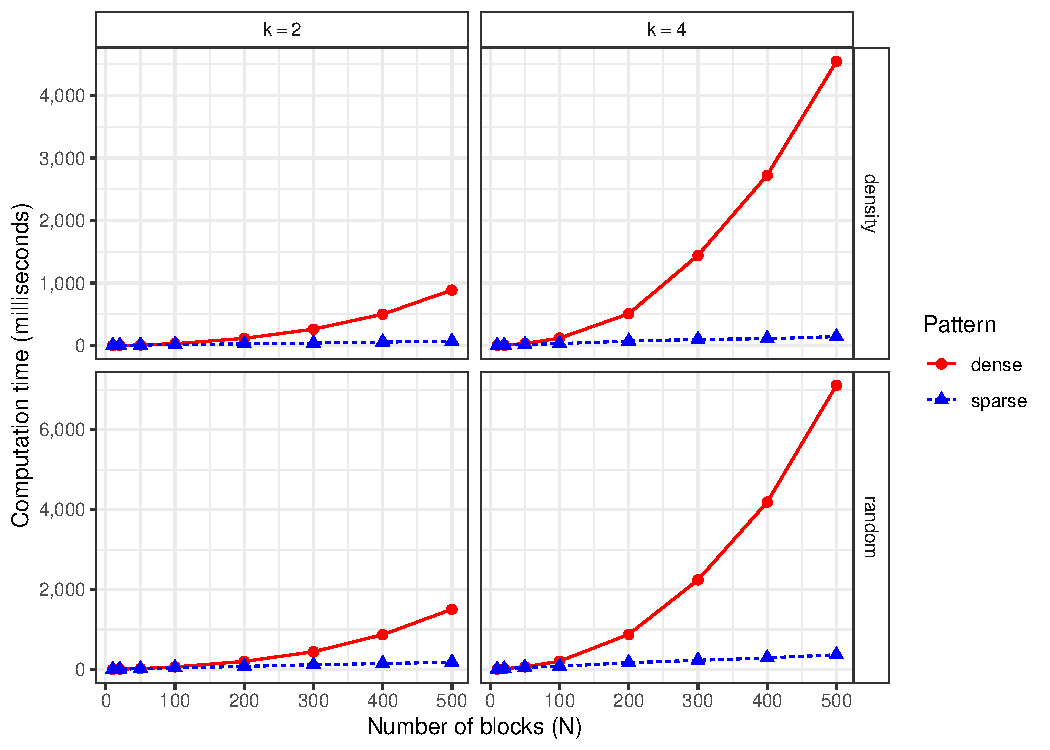
\includegraphics[width=\maxwidth]{figure/unnamed-chunk-14-1} \end{Schunk}
\caption{Mean computation time for simulating 1,000 MVN samples, and
  computing 1,000 MVN densities, averaged over 200 replications.
  Densities were computed using \func{dmvnorm} and
  \func{dmvn.sparse}, while random samples were generated using
  \func{rmvnorm} and \func{rmvn.sparse}.}\label{fig:densRand}
\end{figure}

The \func{sparseMVN} functions always require a sparse Cholesky decomposition
of the covariance or precision matrix, and the \pkg{mvtnorm} functions
require a dense precision matrix to be inverted into a dense covariance matrix.
Figure \ref{fig:cholSolve} compares the computation times of these
preparatory steps.  There are three cases to consider:  inverting a dense matrix using the \func{solve}
function, decomposing a sparse matrix using \func{Cholesky}, and
decomposing a dense matrix using \func{chol}.  Applying \func{chol} to
a dense function is not a required operation in advance of calling
\func{rmvnorm} or \func{dmvnorm}, but those functions will invoke some
kind of decomposition internally.  We include it in our comparison because it comprises
a substantial part of the computation time.  The decomposition and
inversion operations on the dense matrices grow cubically as the size of
the matrix increases.  The sparse Cholesky decomposition time is
negligible. For example, the mean run time for the $N=500$,
$k=4$ case is about 0.39 ms.

\begin{figure}[tb]
\begin{Schunk}

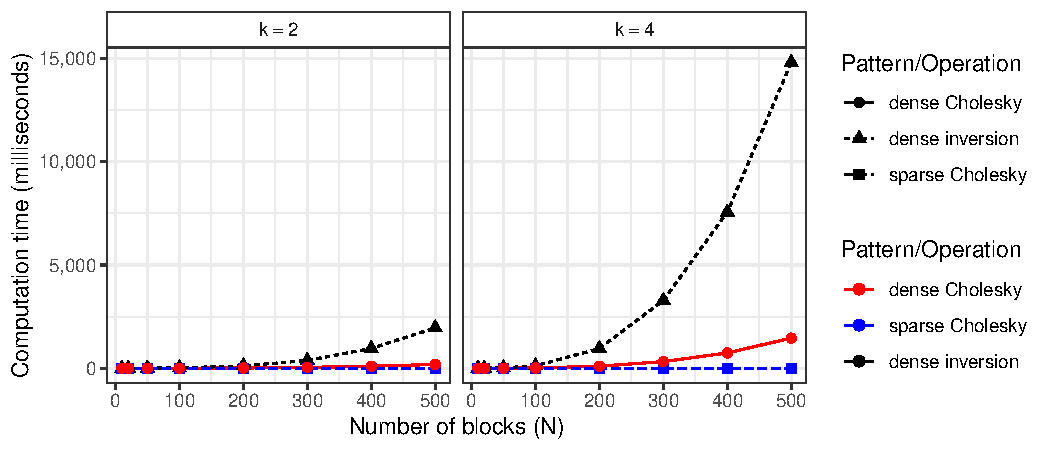
\includegraphics[width=\maxwidth]{figure/unnamed-chunk-15-1} \end{Schunk}
\caption{Computation time for Cholesky decomposition of sparse and
  dense matrices, and inversion of dense matrices.}\label{fig:cholSolve}
\end{figure}

Code to replicate the data used in Figures~\ref{fig:densRand} and \ref{fig:cholSolve}
is available as an online supplement to this paper, and in the
\func{doc/} directory of the installed package.



\FloatBarrier
\bibliography{sparseMVN}

\end{document}
